\chapter{Ewolucyjne techniki optymalizacji}
\label{cha:genetyczne}
Algorytmami ewolucyjnymi nazywne są algorytmy, które w celu przeszukania przestrzeni rozwiązań  wykorzystują mechanizmy zaczerpnięte ze zjawiska ewolucji biologicznej. Jest to ogólna nazwa dla metod takich jak algorytmy ewolucyjne, strategie ewolucyjne czy neuroewolucje. Przykładowe rozwiązania danego problemu reprezentowane są przez genotypy osobników. Finalne rozwiązanie wybierane jest spośród genotypów wszystkich osobników w danej populacji. Poniższy rozdział stanowi wprowadzenie do algorytmów ewolucyjnych, których najbardziej popularnym rodzajem są algorytmy genetyczne. 

\section{Algorytmy ewolucyjne}
\label{sec:historiagenetycznych}
Algorytmy ewolucyjne przetwarzają populację osobników reprezentujących potencjalne rozwiązania zadania. Populacja generowana jest losowo, wraz z pewnym zestawem cech dla każdego osobnika nazywanym w algorytmach genetycznych genotypem. Genotyp jest takim zestawem cech, który umiejscawia go w pewnej przestrzeni rozwiązań, co umożliwia jego ewaluację. Podczas działania algorytmu, nowe osobniki tworzone są poprzez krzyżowanie się istniejących, najgorzej przystosowane umierają, a poprzez mutację wpływają na genotypy.  

Na przestrzeni lat zostało zaproponowanych wiele algorytmów bazujących na mechanizmach genetycznych, jednak wszystkie z nich opierały się na tych samych bazowych mechanizmach. Każdy z osobników populacji mógł, zmieniając swój genotyp, przybliżyć całą populację do znalezienia optymalnego rozwiązania postawionego problemu. Większość współczesnych rozwiązań stosuje również krzyżowanie się osobników, jako drugą główną składową działania algorytmów tego typu.

Początki algorytmów ewolucyjnych sięgają lat 50. XX wieku \cite{GA1}, jednak ich idee nie były rozwijane przez wiele lat, głównie ze względu na ograniczenia sprzętowe, jak i metodologiczne. Dopiero dwadzieścia lat później \cite{GA2} pojawiły się prace rozwijające modele ewolucyjne. Wtedy też zostało zaproponowane twierdzenie Hollanda o schematach, które uważane jest za podstawę wyjaśnienia algorytmów ewolucyjnych. 

Znaczącą kwestią wpływającą na tempo rozwoju algorytmów ewolucyjnych było użycie techniki uwzględniającej ewolucję zarówno przez mutację, jak i krzyżowanie się osobników z danej populacji. Podczas kolejnych lat badań, algorytmy tego typu zostały poszerzone o kod genetyczny pozwalający reprezentować strukturę każdego problemu.


\begin{figure}[H]
\begin{center} 
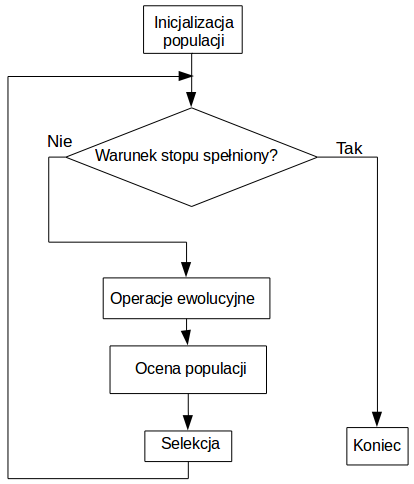
\includegraphics[scale=0.6]{tresc/pics/GAdiagram.png}
\caption{Diagram blokowy klasycznego algorytmu ewolucyjnego}
\label{fig:GAdiagram}
\end{center}
\end{figure}

Klasyczne algorytmy ewolucyjne działają zgodnie z algorytmem przedstawionym na diagramie \ref{fig:GAdiagram}. Początkowo inicjalizowana jest losowa populacja, która aż do spełnienia warunku stopu, oddziałuje na siebie zgodnie z pewnymi zasadami. Warunkiem stopu, podobnie jak w algorytmie roju cząstek, może być osiągnięcie limitu iteracji lub zadowalającego wyniku. Podczas każdej iteracji z całej populacji wybierana jest część osobników, która zostanie poddana krzyżowaniu się między sobą. Następnie te osobniki poddawane są mutacji. Dla każdego z nich wyliczana jest funkcja przystosowania pozwalająca ocenić jakość jego genotypu.


\section{Ewolucyjny system wieloagentowy}
\label{cha:pyage}
EMAS (ang. Evolutionary Multi-Agent System) jest paradygmatem obliczeniowym zaproponowanym w 1996 roku \cite{emas1}. Jest to połączenie algorytmu ewolucyjnego z systemem wieloagentowym. Idea algorytmu opiera się na koncepcji, która mówi, że agenci w środowisku mogą się spotykać, reprodukować, mutować i umierać.  


\subsection*{Agent i system wieloagentowy}

W roku 1997 została zaproponowana definicja agenta, która definiuje go jako ,,system, który usytuowany jest w pewnym środowisku, i którego jednocześnie jest częścią; agent obserwuje (odbiera, odczuwa) to środowisko oraz działa w nim: w czasie, według własnego planu, wpływając na to, co będzie mógł zaobserwować w przyszłości'' \cite{opisagenta}. Definicja powstała na skutek wnikliwej analizy różnych podejść agentowości.

Zgodnie ze znajdującą się powyżej definicją, za najistotniejsze cechy agenta należy uznać \cite{agentowyemas}:
\begin{itemize}
\item usytuowanie - agent jest częścią środowiska, w którym się znajduje
\item autonomia - agent ma pełną kontrolę nad swoim stanem wewnętrznym oraz akcjami
\item reaktywność - agent postrzega środowisko i zmiany zachodzące w nim i reaguje na nie
\item zdolności socjalne - agent współdziała z innymi agentami
\end{itemize}

System agentowy to system komputerowy, którego główną abstrakcją jest pojęcie agenta \cite{systemagentowy}. System składający się z wielu współdziałających agentów nazywany jest systemem wieloagentowym. Interakcje między agentami, mogące przyjąć formę kooperacji, koordynacji bądź negocjacji są najistotniejszą cechą charakterystyczną tej klasy systemów i stanowią o ich sile. 



\subsection*{Koncepcja EMAS}
\label{sec:emas}

Podczas pracy EMAS, w przeciwieństwie do klasycznego algorytmu ewolucyjnego, nie jest wymagana żadna globalna wiedza o problemie, wszystkie obliczenia są zdecentralizowane. Agenci są niezależni oraz zdolni do podejmowania własnych decyzji dotyczących ich akcji. Wykorzystywanie takich struktur organizacji agentów jak wyspy obliczeniowe pozwala na łatwą skalowalność algorytmu. 

Dziedziczenie i selekcja to dwa główne elementy algorytmów ewolucyjnych, które w algorytmie EMAS realizowane są za pomocą zjawisk reprodukcji i śmierci. Agenci o najlepszym przystosowaniu są zachowani i mogą produkować swoje potomstwo. Agenci o najgorszych parametrach są całkowicie usuwani z otoczenia. Takie zachowanie zmusza populację do ewolucji oraz w każdym kroku zbliża ją do lokalnego ekstremum \cite{emas2}.

Każdy z agentów posiada energię, która warunkuje wykonywane przez niego akcję. Jeśli energia agenta spadnie do zera, oznacza to jego śmierć i skutkuje usunięciem z populacji. Energia jest wymieniana przez agentów podczas spotkań. Agent z mniejszym poziomem dopasowania oddaje swoją energię agentowi z większym poziomem dopasowania.

\subsection*{Agent w EMAS}
\label{sec:agentgenetyczny}
Każdy z agentów charakteryzuje się trzema parametrami:
\begin {itemize}
\item genotyp (ang. genotype)
\item dopasowanie (ang. fitness)
\item energia (ang. energy)
\end {itemize}
Genotyp agenta jest pojedynczą instancją rozwiązania zadanego problemu populacji. Jest to podstawa do obliczenia dopasowania. Genotyp jest cechą dziedziczoną podczas reprodukcji i może ulec jednorazowej mutacji podczas powstawania agenta.

Kolejną cechą jest dopasowanie, które jest liczbą reprezentującą jakość genotypu. Lepsze genotypy mają lepsze wartości dopasowania i mają większe prawdopodobieństwo aby być wybranym przy procesie reprodukcji, ponieważ najczęściej osobniki z najlepszym genotypem mają najwyższą wartość energii (warunkującej reprodukcję osobnika). Wartość dopasowania obliczana jest na podstawie genotypu. Dopasowanie danego agenta, tak samo jak jego genotyp, nie zmienia sie w czasie jego życia.

Ostatnią cechą wpływającą na sposób selekcji jest energia. Ze względu na brak globalnej wiedzy agentów, nie jest możliwa ocena ich wszystkich w tym samym czasie. Ponieważ proces ewolucji jest asynchroniczny, metody selekcji znane z klasycznych algorytmów ewolucyjnych nie mogły zostać użyte. Z tego powodu została wprowadzona energia. Można opisać ten parametr jako stan agenta. Podczas spotkań agent może energię zyskiwać lub tracić, zależnie od jakości jego genotypu (czyli wartości dopasowania). Agenci z lepszym genotypem są bardziej skłonni do gromadzenia energii. Całkowita ilość energii w populacji jest stała.

Ponieważ agenci w algorytmie EMAS są całkowicie autonomiczni, decyzję o swoim zachowaniu podejmują na podstawie poziomu energii. Jeśli jej liczba przekracza pewien próg, to mogą się reprodukować, a jeśli osiągnie zero, to agent umiera \cite{emas3}. Energia wymieniana jest podczas spotkań agentów.


\subsection*{Interakcje agentów}
Istnieją trzy możliwe działania agenta, które może podjąć w danym kroku iteracji:
\begin{itemize} 
\item śmierć (ang. death) 
\item reprodukcja (ang. reproduction) 
\item spotkanie (ang. meeting) 
\item migracja (ang. migration)
\end{itemize}

Śmierć to usunięcie agenta z populacji, spowodowane jest poprzez osiągnięcie przez danego agenta zerowego poziomu energii.

Reprodukcja jest procesem tworzenia nowych agentów. Wymaga wystąpienia jednego lub dwójki rodziców i skutkuje jednym nowopowstałym agentem. W przypadku zaistnienia dwójki rodziców, potomek ma cechy będące pochodną obojga z nich. Jak zostało wspomniane w rozdziale, rozwiązanie oraz dopasowanie są stałe podczas życia agenta, więc ich wartość u rodziców się nie zmienia. Jedyną zmianą parametru jest zmniejszenie ich poziomu energii, która jest przekazywana nowopowstałym agentom. Genotypy nowonarodzonych agentów są tworzone poprzez wykorzystanie genotypów ich rodziców.

Spotkanie jest działaniem pozwalającym na wymianę energii. Dzięki niemu agenci o lepszej wartości dopasowania są w stanie pobrać energię od tych z gorszą. Spotkanie sprowadza się do porównania dopasowania dwóch agentów i w jego efekcie transferu energii. Jest to szybki sposób porównania i nagradzania najlepszych rozwiązań. Jak zostało wspomniane wcześniej, ilość energii jest stała w całym systemie.

%\subsection{Sąsiedztwo agentów}
Wszystkie akcje, jakie agenci mogą pomiędzy sobą wykonać mogą zaistnieć wyłącznie wtedy, gdy agenci sąsiadują ze sobą. Pod koniec każdej z iteracji następuje przemieszczenie się, migracja agentów. Pozwala to na uniknięcie ciągłej interakcji tych samych agentów ze sobą.

%\begin{figure}[H]
%\begin{center} 
%\includegraphics[scale=0.6]{tresc/pics/emasdiagram.png}
%\caption{Akcje agentów w algorytmie EMAS}
%\label{fig:emasdiagram}
%\end{center}
%\end{figure}

\subsection*{Struktura populacji}
Populacją nazywany jest cały zbiór agentów, jej początkowy rozmiar jest parametryzowany i zmienia się w czasie wykonywania programu.

Podczas pojedynczego przebiegu programu można podzielić populację na grupy nazywane wyspami \cite{emas3}, na których populacje (ich liczebność, jakość) zmieniają się niezależnie od siebie w tym samym czasie. Zaistnienie migracji agenta pomiędzy wyspami możliwe jest po przekroczeniu pewnego poziomu jego energii, który jest parametrem wejściowym dla algorytmu.

Poprzez wprowadzenie migracji między różnymi wyspami, możliwe jest eksportowanie pewnych rozwiązań pomiędzy nimi. Ma to pozytywny wpływ na minimalizowanie tendencji populacji do wpadania w lokalne ekstrema poprzez zwiększenie różnorodności. Dobre rozwiązanie opracowane w jednej populacji może być wprowadzone do innej, co sprzyja różnorodności przykładowych rozwiązań. 

Istnienie tego typu rozwiązania może wpłynąć na zrównoleglenie, a co za tym idzie - na czas działania algorytmu. Niezależne od siebie wyspy obliczeniowe można bowiem uruchomić na osobnych węzłach obliczeniowych.



